%% ============================================================
%%  DERMA-GUARD: Risk-Controlled, Cost-Aware Evidence Acquisition
%%  and Deferral for Multimodal Dermatology AI
%%  IEEE Two-Column Format — Overleaf Ready
%%  Version: 2.0  |  Based on Project Specification v2.0
%% ============================================================

\documentclass[conference]{IEEEtran}

%% ── Packages ──────────────────────────────────────────────────
\usepackage[T1]{fontenc}
\usepackage[utf8]{inputenc}
\usepackage{amsmath,amssymb,amsthm}
\usepackage{mathtools}
\usepackage{bm}
\usepackage{graphicx}
\usepackage{booktabs}
\usepackage{multirow}
\usepackage{array}
\usepackage{tabularx}
\usepackage{xcolor}
\usepackage{colortbl}
\usepackage{url}
\usepackage{hyperref}
\usepackage{cite}
\usepackage{balance}
\usepackage{algorithm}
\usepackage{algorithmic}
\usepackage{subcaption}
\usepackage{tikz}
\usetikzlibrary{shapes.geometric,arrows.meta,positioning,fit,backgrounds,calc}
\usepackage{pgfplots}
\pgfplotsset{compat=1.18}
\usepackage{enumitem}
\usepackage{microtype}
\usepackage{float}

%% ── Color palette ─────────────────────────────────────────────
\definecolor{dermblue}{RGB}{13,71,161}
\definecolor{dermred}{RGB}{183,28,28}
\definecolor{dermgreen}{RGB}{27,94,32}
\definecolor{dermgold}{RGB}{230,174,8}
\definecolor{dermgray}{RGB}{66,66,66}
\definecolor{rowhl}{RGB}{232,240,254}
\definecolor{bestrow}{RGB}{200,230,201}

%% ── Theorem environments ──────────────────────────────────────
\newtheorem{theorem}{Theorem}
\newtheorem{proposition}{Proposition}
\newtheorem{definition}{Definition}
\newtheorem{remark}{Remark}

%% ── Math operators ────────────────────────────────────────────
\DeclareMathOperator*{\argmin}{arg\,min}
\DeclareMathOperator{\JS}{JS}
\newcommand{\R}{\mathbb{R}}
\newcommand{\E}{\mathbb{E}}
\newcommand{\1}{\mathbf{1}}
\newcommand{\calR}{\mathcal{R}}
\newcommand{\calC}{\mathcal{C}}

%% ── Hyperref setup ────────────────────────────────────────────
\hypersetup{
  colorlinks=true,
  linkcolor=dermblue,
  citecolor=dermblue,
  urlcolor=dermblue
}

\IEEEoverridecommandlockouts

% ============================================================
\begin{document}

%% ── Title block ───────────────────────────────────────────────
\title{\textbf{DERMA-GUARD}: Risk-Controlled, Cost-Aware Evidence
  Acquisition and Deferral for Multimodal Dermatology AI}

\author{%
  \IEEEauthorblockN{Member 1\IEEEauthorrefmark{1},
                    Member 2\IEEEauthorrefmark{1},
                    Member 3\IEEEauthorrefmark{1}}
  \IEEEauthorblockA{\IEEEauthorrefmark{1}%
    Department of Computer Science and Engineering,
    [Institution Name], [City, Country]\\
    \texttt{\{member1, member2, member3\}@institution.edu}}
}

\maketitle

%% ── Abstract ─────────────────────────────────────────────────
\begin{abstract}
We present \textbf{DERMA-GUARD}, a multimodal dermatology research platform
that addresses the clinically motivated decision: given a clinical close-up
photograph of a skin lesion, should an AI system \emph{answer now},
\emph{request a dermoscopic image}, or \emph{defer to a human}---and can it
make this choice with a statistical guarantee on its malignancy miss rate?
The system computes calibrated class probabilities, predictive uncertainty
via deep ensembles, cross-modal consistency scores, input-quality estimates,
and out-of-distribution (OOD) signals. An \textbf{Evidence-Adaptive Decision
Engine (EADE)} applies an expected-loss minimisation rule over a clinically
asymmetric cost matrix. Decision thresholds are calibrated using
\textbf{Learn-then-Test (LTT) / conformal risk control}, providing a
finite-sample bound: the malignancy miss rate on auto-proceeded cases is
$\leq\!\alpha$ with probability $\geq\!1-\delta$ under exchangeability.
We evaluate on \textbf{MILK10k} (5,240 paired lesions, $\approx$96\%
histopathology-confirmed), compare against eight baselines---including
HOT-style dermoscopy-on-uncertainty rules, learning-to-defer, oracle
acquisition, and confidence-threshold abstention---and stress-test through
\textbf{DERMA-STRESS}: seven failure families covering image degradation,
missing modalities, contradictory metadata, distribution shift,
leave-class-out OOD, combined failures, and operational failures. We
additionally measure \emph{where the statistical guarantee breaks} under
distribution shift---a core reported finding. Subgroup analysis across six
skin-tone levels uses group-conditional conformal calibration. Results are
reported honestly; the method may or may not outperform all baselines.

\vspace{2pt}
\textit{Index Terms}---Dermatology AI, selective prediction, conformal
prediction, active feature acquisition, evidence deferral, cost-aware
decision making, multimodal fusion, OOD detection, fairness in AI.
\end{abstract}

% ============================================================
\section{Introduction}
\label{sec:introduction}
% ============================================================

Skin cancer is among the most prevalent malignancies worldwide, yet early
detection through visual inspection dramatically improves outcomes
\cite{tschandl2018ham10000}. Clinical close-up photographs are cheap and
ubiquitous; dermoscopy yields higher diagnostic accuracy but requires
specialised equipment and a trained operator \cite{muller2026complementary}.
A recent reader study on the MILK10k dataset \cite{tschandl2024milk10k}
showed that the two modalities carry \emph{complementary} information:
dermoscopy alone gave higher sensitivity for malignant lesions, while
clinical close-ups gave higher specificity. This complementarity creates a
natural three-way decision for any automated screening system:

\begin{enumerate}[leftmargin=*, label=(\arabic*)]
  \item \textbf{PROCEED}---answer immediately from the available clinical
        image, accepting its inherent risk.
  \item \textbf{ACQUIRE}---request the dermoscopic image when its expected
        benefit exceeds its acquisition cost.
  \item \textbf{DEFER}---route to human review when evidence is
        insufficient regardless of further acquisition.
\end{enumerate}

Existing work addresses \emph{parts} of this problem.
\textit{Selective classification} \cite{geifman2017selective} studies
abstention but not active acquisition. \textit{HOT} \cite{mehta2023hot}
recommends dermoscopy when the clinical image is deemed insufficient but
lacks an explicit cost model and a \emph{statistical} risk guarantee.
Active feature acquisition \cite{shim2018joint,valancius2023aco,rheude2025cama}
addresses test-time modality selection under budgets. Conformal prediction
\cite{angelopoulos2021gentle,angelopoulos2020raps} provides distribution-free
coverage guarantees. Learning-to-defer \cite{mozannar2020defer} allocates
cases between model and expert. \textbf{What is not established in the
dermatology literature we have reviewed} is a policy that (a) jointly decides
proceed/acquire/defer under an explicit cost model, (b) carries a
finite-sample risk guarantee on malignancy miss rate, and (c) is stress-tested
under combined evidence failures with the guarantee's breakdown quantified.

\medskip
\noindent\textbf{Central research question.} Can a cost-aware,
risk-controlled acquire/defer policy achieve a better
reliability--coverage--cost trade-off than confidence-threshold abstention,
learning-to-defer \cite{mozannar2020defer}, and HOT-style dermoscopy
recommendation---on clean data \emph{and} under controlled evidence failures?

\medskip
\noindent\textbf{Contributions.}
\begin{enumerate}[leftmargin=*, label=\textbf{C\arabic{enumi}.}]
  \item \textbf{EADE:} An expected-loss minimisation policy with a
        conformal/LTT safety layer that bounds malignancy miss rate
        on auto-proceeded cases with probability $\geq 1-\delta$.
  \item \textbf{DERMA-STRESS:} A versioned, reproducible stress-test
        protocol across seven failure families, including the first
        systematic measurement of guarantee violation under distribution
        shift in a dermatology setting.
  \item \textbf{Acquisition analysis:} An acquisition-value estimator
        evaluated against oracle and random bounds, with two
        project-defined diagnostic metrics (MSES and NIR).
  \item \textbf{Fairness analysis:} Group-conditional conformal
        calibration across six skin-tone levels using MILK10k metadata.
\end{enumerate}

\medskip
\noindent\textbf{Disclaimer.} This is a research prototype, not a medical
device. All hypotheses are predictions; results are reported
unconditionally including negative findings.

% ============================================================
\section{Related Work}
\label{sec:related}
% ============================================================

\subsection{Multimodal Dermatology}

Early multimodal systems combined dermoscopy with metadata
\cite{kawahara2019derm7pt}. DermFormer \cite{dermformer2025} applies nested
multi-modal Vision Transformers (ViTs) to clinical images, dermoscopic images,
and metadata. CosCatNet / Zuo et al.\ \cite{zuo2025coscatnet} uses adaptive
uncertainty-aware fusion for multi-label classification. JI-ADF
\cite{jiadf2025} performs joint-individual learning with adaptive decision
fusion on MILK10k; its reported results serve as our primary fusion reference
on the same dataset (labelled \texttt{paper-reported}). PanDerm
\cite{panderm2025} is a dermatology foundation model considered as an optional
backbone subject to licence and compute verification.

\subsection{Selective Prediction and Calibration}

Selective classification \cite{geifman2017selective} abstains when confidence
falls below a threshold. The Area Under the Risk--Coverage curve (AURC) is a
standard metric, but Traub et al.\ \cite{traub2024augrc} identify flaws and
propose AUGRC---the Area Under the \emph{Generalised} Risk--Coverage curve---
which we adopt as our primary multi-threshold metric. Calibration via
temperature scaling \cite{guo2017calibration} corrects overconfident deep
networks. Deep ensembles \cite{lakshminarayanan2017ensembles} provide
epistemic uncertainty through prediction diversity.

\subsection{Conformal Prediction}

Conformal prediction \cite{angelopoulos2021gentle} constructs label sets
$\mathcal{C}_\alpha(x)$ with marginal coverage $\geq 1-\alpha$. RAPS/APS
\cite{angelopoulos2020raps} are efficient set-construction methods.
\textbf{Learn-then-Test (LTT)} \cite{angelopoulos2021ltt} and
\textbf{conformal risk control} \cite{angelopoulos2022crc} extend coverage
to general losses. Fayyad et al.\ \cite{fayyad2023conformal} evaluate
conformal prediction for skin-lesion classification; our work differs by
\emph{driving actions} with conformal sets rather than using them purely for
uncertainty quantification. Zoravar et al.\ \cite{zoravar2025conformal}
study conformal prediction under domain shift in dermatology, informing our
guarantee-violation analysis.

\subsection{Active Feature and Modality Acquisition}

Shim et al.\ \cite{shim2018joint} use RL for joint active feature
acquisition and classification. CAMA \cite{rheude2025cama} performs
cohort-based active modality acquisition under budget constraints. ACO
\cite{valancius2023aco} proposes an acquisition-conditioned oracle for
non-greedy active feature acquisition. SAGEAgent \cite{sageagent2026} uses
an LLM agent for cost-aware sequential modality acquisition in a
non-dermatology setting. Our work differs by focusing on binary
acquire/defer in dermatology with a finite-sample guarantee.

\subsection{Learning to Defer}

Mozannar and Sontag \cite{mozannar2020defer} propose a consistent surrogate
for learning-to-defer (L2D), which jointly trains a classifier and a
deferral rule. We implement L2D as a strong baseline (B4).

\subsection{OOD Detection}

Energy-based OOD \cite{liu2020energy} computes $E(x)=-T\log\sum_k e^{f_k(x)/T}$.
Mahalanobis distance \cite{lee2018mahalanobis} operates on
penultimate-layer features. Both are evaluated and combined with conformal
sets for the safety layer.

\subsection{Fairness in Medical AI}

Lu et al.\ \cite{lu2021fair} propose group-conditional conformal predictors
for medical imaging. We adopt this approach for skin-tone subgroup
calibration using MILK10k's six-level skin-tone metadata.

\subsection{HOT: The Closest Threat to Novelty}

HOT \cite{mehta2023hot} applies a hierarchical prediction pipeline that
alerts on OOD clinical images, recommends dermoscopy when uncertain, and
fuses both when available. HOT does \emph{not} (a) use an explicit cost
model, (b) provide a finite-sample malignancy miss-rate guarantee, or
(c) measure guarantee violation under distribution shift. We implement a
HOT-style baseline (B5) and clearly position our additional contributions.

\medskip
Table~\ref{tab:comparison} summarises key distinctions between DERMA-GUARD
and closely related prior work.

\begin{table*}[t]
  \centering
  \caption{%
    Comparison of DERMA-GUARD with closely related systems.
    \checkmark\,= present; $\circ$\,= partial; --\,= absent.
    Results labelled \texttt{paper-reported} or \texttt{our-reimplementation}.
  }
  \label{tab:comparison}
  \renewcommand{\arraystretch}{1.25}
  \setlength{\tabcolsep}{4pt}
  \small
  \begin{tabularx}{\linewidth}{%
      >{\bfseries}l
      >{\centering\arraybackslash}X
      >{\centering\arraybackslash}X
      >{\centering\arraybackslash}X
      >{\centering\arraybackslash}X
      >{\centering\arraybackslash}X
      >{\centering\arraybackslash}X
      >{\centering\arraybackslash}X
      >{\centering\arraybackslash}X}
    \toprule
    \textbf{System}
      & \textbf{Paired Modalities}
      & \textbf{Acquire Action}
      & \textbf{Defer Action}
      & \textbf{Cost Model}
      & \textbf{Risk Guarantee}
      & \textbf{Stress Tests}
      & \textbf{Fairness}
      & \textbf{Dataset} \\
    \midrule
    HOT \cite{mehta2023hot}
      & \checkmark & \checkmark & -- & -- & -- & -- & -- & Private \\
    JI-ADF \cite{jiadf2025}
      & \checkmark & -- & -- & -- & -- & -- & -- & MILK10k \\
    DermFormer \cite{dermformer2025}
      & \checkmark & -- & -- & -- & -- & $\circ$ & -- & ISIC \\
    Fayyad et al.\ \cite{fayyad2023conformal}
      & -- & -- & -- & -- & CP coverage & -- & -- & ISIC/Ham \\
    Zoravar et al.\ \cite{zoravar2025conformal}
      & -- & -- & -- & -- & CP~+~shift & -- & -- & ISIC \\
    CAMA \cite{rheude2025cama}
      & \checkmark & \checkmark & -- & \checkmark & -- & -- & -- & Non-derm \\
    L2D \cite{mozannar2020defer}
      & -- & -- & \checkmark & -- & -- & -- & -- & General \\
    \rowcolor{bestrow}
    \textbf{DERMA-GUARD (ours)}
      & \checkmark & \checkmark & \checkmark & \checkmark
      & \checkmark\,(LTT) & \checkmark\,(7 fams.) & \checkmark & MILK10k \\
    \bottomrule
  \end{tabularx}
\end{table*}

% ============================================================
\section{Problem Formulation}
\label{sec:formulation}
% ============================================================

\subsection{Notation}

Table~\ref{tab:notation} defines the notation used throughout the paper.

\begin{table}[H]
  \centering
  \caption{Notation summary.}
  \label{tab:notation}
  \renewcommand{\arraystretch}{1.15}
  \small
  \begin{tabular}{cl}
    \toprule
    \textbf{Symbol} & \textbf{Meaning} \\
    \midrule
    $x^c$ & Clinical close-up image \\
    $x^d$ & Dermoscopic image \\
    $z$   & Structured metadata (age, sex, site, skin tone) \\
    $S \subseteq \{c, d, z\}$ & Currently available evidence subset \\
    $y \in \{1,\ldots,K\}$ & Diagnostic class \\
    $g(y) \in \{\text{B}, \text{M}\}$ & Malignancy grouping \\
    $p_S(y \mid x_S)$ & Calibrated posterior using evidence $S$ \\
    $L(y, \hat{y})$ & Loss of predicting $\hat{y}$ when truth is $y$ \\
    $c_{\text{acq}}(m)$ & Cost of acquiring modality $m$ \\
    $c_{\text{def}}$ & Cost of deferring to a human \\
    $\alpha$ & Target malignancy miss rate ($= 0.05$) \\
    $\delta$ & Failure probability ($= 0.10$) \\
    $\hat{\lambda}$ & LTT-calibrated PROCEED threshold \\
    $T_{\max}$ & Maximum acquisition rounds ($= 1$) \\
    \bottomrule
  \end{tabular}
\end{table}

\subsection{Cost Matrix}

We use a clinically asymmetric cost matrix (Table~\ref{tab:cost}) that
penalises missing a malignancy far more than a false alarm. Values are
pre-registered before the final test run; sensitivity analysis across
$\ell_{\text{miss}} \in \{5,10,20\}$ is mandatory.

\begin{table}[H]
  \centering
  \caption{%
    Pre-registered asymmetric cost matrix.
    $\ell_{\text{sub}}=1$, $\ell_{\text{miss}}=10$, $\ell_{\text{fa}}=2$ (default).
  }
  \label{tab:cost}
  \renewcommand{\arraystretch}{1.2}
  \small
  \begin{tabular}{lcccc}
    \toprule
    \textbf{Truth$\backslash$Pred.}
      & \textbf{Correct}
      & \textbf{Wrong, same grp.}
      & \textbf{Benign for Mal.}
      & \textbf{Mal.\ for Benign} \\
    \midrule
    Loss & $0$ & $\ell_{\text{sub}}$ & $\ell_{\text{miss}}$ & $\ell_{\text{fa}}$ \\
    Default & $0$ & $1$ & $\mathbf{10}$ & $2$ \\
    \bottomrule
  \end{tabular}
\end{table}

\subsection{Action Space}

The system selects one action per case:
$a \in \mathcal{A} = \{\texttt{PROCEED},\;\texttt{ACQUIRE}(m),\;\texttt{DEFER}\}.$
\texttt{ACQUIRE}$(m)$ requests only modalities that are \emph{actually available}.
The loop halts after $T_{\max}=1$ round or when \texttt{DEFER} is triggered.

% ============================================================
\section{Method}
\label{sec:method}
% ============================================================

\subsection{Expected-Loss Decision Rule}

\paragraph{PROCEED.}
The Bayes-optimal expected loss of proceeding:
\begin{equation}
  R_{\text{proc}}(S) = \min_{\hat{y}} \sum_{y} p_S(y \mid x_S)\, L(y, \hat{y}).
  \label{eq:Rproc}
\end{equation}

\paragraph{ACQUIRE.}
Acquiring modality $m \notin S$ reduces expected proceed-loss by the
acquisition-value estimate $h_m(x_S)$:
\begin{equation}
  R_{\text{acq}}(S, m) = R_{\text{proc}}(S) - h_m(x_S) + c_{\text{acq}}(m).
  \label{eq:Racq}
\end{equation}

\paragraph{DEFER.}
\begin{equation}
  R_{\text{def}} = c_{\text{def}}.
  \label{eq:Rdef}
\end{equation}

\paragraph{Raw policy.}
\begin{equation}
  a_{\text{raw}}(S) = \argmin\Bigl\{
    R_{\text{proc}}(S),\;
    \min_{m \in \mathcal{M}_{\text{avail}}\setminus S} R_{\text{acq}}(S,m),\;
    R_{\text{def}}
  \Bigr\}.
  \label{eq:policy_raw}
\end{equation}

\subsection{Acquisition-Value Estimator}

The estimator $h_d(x_S)$ predicts the loss reduction from adding dermoscopy,
trained on \emph{out-of-fold} targets to prevent optimistic bias:

\begin{enumerate}[leftmargin=*, label=\textbf{Step \arabic*.}]
  \item Run 5-fold CV to produce held-out posteriors $p_{\{c,z\}}$ and
        $p_{\{c,d,z\}}$ for every training lesion.
  \item Target: $t_i = R_{\text{proc}}(\{c,z\})_i - R_{\text{proc}}(\{c,d,z\})_i$
        (realised loss reduction from adding dermoscopy).
  \item Fit $h_d$ (LightGBM or small MLP) on pre-acquisition features:
        clinical-model posterior, predictive entropy $H[\bar{p}]$, mutual
        information MI, quality scores, OOD score, metadata.
  \item At test time: $\hat{\E}[R_{\text{proc}}(S\cup\{d\})] = R_{\text{proc}}(S) - h_d(x_S)$.
\end{enumerate}

\noindent\textbf{Fallback baselines:} acquire iff $H[\bar{p}] > \tau$
(HOT-style; B5), acquire iff MI $> \tau$ (greedy information gain; B6).

\subsection{Calibration and Uncertainty}

\paragraph{Temperature scaling \cite{guo2017calibration}.}
A single scalar $T$ is fit per modality configuration on the validation
split: $\tilde{p}_k = e^{f_k/T} / \sum_j e^{f_j/T}$.

\paragraph{Deep ensemble \cite{lakshminarayanan2017ensembles}.}
$M=3$ seeds, averaged: $\bar{p}(y)=\frac{1}{M}\sum_j p_j(y)$.
\begin{align}
  H[\bar{p}] &= -\sum_y \bar{p}(y)\log\bar{p}(y), \label{eq:entropy}\\
  \text{MI}  &= H[\bar{p}] - \tfrac{1}{M}\textstyle\sum_j H[p_j]. \label{eq:mi}
\end{align}

\paragraph{Consistency signal (Member 2).}
Jensen--Shannon divergence between modality-specific posteriors:
\begin{equation}
  \JS(p_{\{c\}} \,\|\, p_{\{z\}}) =
    \tfrac{1}{2}\text{KL}(p_{\{c\}} \| m) +
    \tfrac{1}{2}\text{KL}(p_{\{z\}} \| m),\quad
  m = \tfrac{1}{2}(p_{\{c\}}+p_{\{z\}}).
  \label{eq:js}
\end{equation}
Rule-based contradiction flags supplement continuous JS when metadata fields
conflict with extracted symptom text.

\paragraph{OOD scores.}
Energy score \cite{liu2020energy}:
$E(x) = -T\log\sum_{k} e^{f_k(x)/T}.$
Mahalanobis distance \cite{lee2018mahalanobis} on penultimate features:
$d_M(x) = \sqrt{(\phi(x)-\mu_{\hat{y}})^\top \Sigma^{-1} (\phi(x)-\mu_{\hat{y}})}.$

\subsection{Safety Layer: Conformal Sets and Learn-then-Test}

\paragraph{Conformal prediction sets.}
Using the calibration split, APS/RAPS sets $\mathcal{C}_\alpha(x_S)$ are
built with marginal coverage $\geq 1-\alpha$. The \textbf{mixed-set rule}:
\begin{equation}
  \texttt{PROCEED} \text{ blocked if } \mathcal{C}_\alpha(x_S) \cap \text{B} \neq \emptyset
  \;\wedge\; \mathcal{C}_\alpha(x_S) \cap \text{M} \neq \emptyset.
  \label{eq:mixed_rule}
\end{equation}
When the conformal set spans both malignancy groups, evidence is
insufficient to auto-proceed.

\paragraph{Learn-then-Test (LTT) \cite{angelopoulos2021ltt}.}
Let $\lambda$ bound how permissive \texttt{PROCEED} is
(e.g.\ a cap on $R_{\text{proc}}$). Define:
\begin{equation}
  \calR(\lambda) = \Pr\bigl(g(y){=}\text{M},\;
    g(\hat{y}){=}\text{B},\; a^*(\lambda){=}\texttt{PROCEED}\bigr).
  \label{eq:risk}
\end{equation}
For a grid $\lambda_1 < \cdots < \lambda_J$ (conservative to permissive):
\begin{enumerate}[leftmargin=*]
  \item Compute empirical risk $\hat{\calR}(\lambda_j)$ on calibration split.
  \item Compute p-value for $H_j:\calR(\lambda_j)>\alpha$
        via the Hoeffding--Bentkus bound or a binomial tail test.
  \item \textbf{Fixed-sequence testing}: walk grid while $p_j\leq\delta$;
        select the most permissive accepted $\hat{\lambda}$.
\end{enumerate}

\begin{theorem}[LTT guarantee \cite{angelopoulos2021ltt}]
With probability $\geq 1-\delta$ over the calibration draw,
$\calR(\hat{\lambda}) \leq \alpha$.
\label{thm:ltt}
\end{theorem}

\begin{remark}
Theorem~\ref{thm:ltt} assumes exchangeability. It does \emph{not} hold
under distribution shift. DERMA-STRESS measures the violation size under
each shift; this measurement is a core reported finding.
\end{remark}

\paragraph{Fairness variant.}
Repeat LTT calibration per skin-tone group $g\in\{1,\ldots,6\}$.
Report coverage and miss rate per group; merge sparse groups ($n<30$);
report sample sizes \cite{lu2021fair}.

\paragraph{Final policy.}
\begin{equation}
  a^*(S) =
  \begin{cases}
    a_{\text{raw}}(S) & \text{if (\ref{eq:mixed_rule}) not triggered}
                        \;\wedge\; R_{\text{proc}}(S) \leq \hat{\lambda},\\
    \texttt{ACQUIRE}(d) & \text{if (\ref{eq:mixed_rule}) triggered}
                          \;\wedge\; d \text{ available,}\\
    \texttt{DEFER} & \text{otherwise.}
  \end{cases}
  \label{eq:final_policy}
\end{equation}
Subject to $T_{\max}=1$ acquisition round (pre-registered).

\begin{algorithm}[t]
\caption{EADE: Evidence-Adaptive Decision Engine}
\label{alg:eade}
\begin{algorithmic}[1]
  \REQUIRE Evidence $S$, calibrated models, LTT threshold $\hat\lambda$,
           conformal sets $\mathcal{C}_\alpha$, cost matrix,
           acquisition estimator $h_d$, available $\mathcal{M}_{\text{avail}}$,
           round counter $t \leftarrow 0$
  \ENSURE  Action $a^*$, reason codes, expected losses
  \WHILE{$t \leq T_{\max}$}
    \STATE Compute $p_S$ via ensemble + temperature scaling
    \STATE Compute $H[\bar p]$, MI, $\JS$, quality, $E(x)$, $d_M(x)$
    \STATE $R_{\text{proc}} \leftarrow \min_{\hat y}\sum_y p_S(y|x_S)L(y,\hat y)$
    \STATE flag $\leftarrow$ mixed-set rule~\eqref{eq:mixed_rule}
    \IF{flag \AND $d \in \mathcal{M}_{\text{avail}}$ \AND $t < T_{\max}$}
      \RETURN \texttt{ACQUIRE}$(d)$, reason=\texttt{CONF\_MIXED}
    \ENDIF
    \IF{$R_{\text{proc}} \leq \hat\lambda$ \AND \NOT flag}
      \RETURN \texttt{PROCEED}, reason=\texttt{EXPECTED\_LOSS\_OK}
    \ENDIF
    \FOR{each $m \in \mathcal{M}_{\text{avail}} \setminus S$}
      \STATE $R_{\text{acq}}(m) \leftarrow R_{\text{proc}} - h_m(x_S) + c_{\text{acq}}(m)$
    \ENDFOR
    \STATE $m^* \leftarrow \argmin_m R_{\text{acq}}(m)$
    \IF{$R_{\text{acq}}(m^*) < \min(R_{\text{proc}}, c_{\text{def}})$
        \AND $t < T_{\max}$}
      \RETURN \texttt{ACQUIRE}$(m^*)$, reason=\texttt{EXPECTED\_LOSS\_GAIN},
              $t \leftarrow t+1$
    \ELSE
      \RETURN \texttt{DEFER}, reason=\texttt{INSUFFICIENT\_EVIDENCE}
    \ENDIF
  \ENDWHILE
  \RETURN \texttt{DEFER}, reason=\texttt{MAX\_ROUNDS}
\end{algorithmic}
\end{algorithm}

% ============================================================
\section{DERMA-STRESS Protocol}
\label{sec:stress}
% ============================================================

DERMA-STRESS is a versioned, reproducible evaluation protocol. Every stress
condition specifies: dataset and split version, corruption type and severity,
random seed, baseline policies and model versions, and saved predictions.

\subsection{Failure Families}

\begin{description}[leftmargin=8pt, labelindent=0pt, style=nextline]
  \item[\textbf{A --- Image degradation.}]
        Gaussian blur, JPEG compression ($Q\in\{10,30,50\}$),
        brightness/contrast shift, downscaling ($4\times,8\times,16\times$),
        motion blur. Applied separately to clinical and dermoscopic branches.

  \item[\textbf{B --- Missing evidence.}]
        Remove dermoscopy; remove metadata fields; remove both.
        Distinguish \texttt{MISSING} from \texttt{PRESENT\_BUT\_LOW\_QUALITY}.

  \item[\textbf{C --- Contradictory context.}]
        Swap anatomic site, shift age bin $\pm 2$ decades, insert
        conflicting symptom text. All changes labelled synthetic;
        no diagnosis leaked.

  \item[\textbf{D --- Distribution shift.}]
        Clinical branch on PAD-UFES-20 \cite{pacheco2020padufes}
        (mapped labels). Centre shift within MILK10k (train on 4 centres,
        test on 1st).

  \item[\textbf{E --- Leave-class-out OOD.}]
        Remove one class (e.g.\ inflammatory, vascular) from training;
        measure deferral rate on held-out examples of that class.

  \item[\textbf{F --- Combined failures.}]
        Degraded clinical + missing metadata; missing dermoscopy + 
        contradictory metadata; distribution shift + degradation;
        unseen class + degradation.

  \item[\textbf{G --- Operational failures.}]
        Inference timeout, worker restart, corrupted upload, LLM provider
        unavailable. Reported separately from diagnostic metrics.
\end{description}

\subsection{Per-Condition Output Metrics}

For each condition: selective risk, coverage, \textbf{AUGRC},
\textbf{guarantee violation} $(\hat{\calR}_{\text{test}} - \alpha)$,
conformal set size, per-skin-tone coverage and miss rate, acquisition rate,
AE$(r)$, deferral rate, latency.

% ============================================================
\section{Experimental Setup}
\label{sec:experiments}
% ============================================================

\subsection{Dataset: MILK10k}

MILK10k \cite{tschandl2024milk10k} contains 5,240 lesions (10,480 images),
each with a paired clinical and dermoscopic image from five centres.
$\approx$96\% histopathology-confirmed. Metadata: age (5-year bins), sex,
site, six-level skin tone, MONET concept probabilities. Eleven diagnostic
categories; rare classes merged for stability.

\paragraph{Splits.} Lesion-level stratified:
$60\%$ train / $15\%$ val / $10\%$ calibration / $15\%$ test (3 seeds).
Patient IDs unavailable; split by ISIC lesion ID; residual leakage
risk stated as a limitation.

\paragraph{Secondary/shift datasets.} Derm7pt \cite{kawahara2019derm7pt}
for replication; PAD-UFES-20 \cite{pacheco2020padufes} for Family D
clinical-branch shift only; HAM10000 \cite{tschandl2018ham10000} for
dermoscopy-branch pretraining or OOD evaluation.

\paragraph{Power note.}
15\% test $\approx$786 lesions ($\approx$50--60 melanomas). Wide CIs
expected for per-class melanoma metrics; binary malignant/benign used
for the guarantee.

\subsection{Model Architecture}

ConvNeXt-Tiny or EfficientNet-B0 (\texttt{timm}, ImageNet pretrained).
Three modality-specific heads trained with modality dropout:
(1) clinical-only $p_{\{c\}}$,
(2) dermoscopy-only $p_{\{d\}}$,
(3) late-fused $p_{\{c,d,z\}}$.
3-seed ensemble; temperature scaling per configuration on validation split.

\subsection{Baselines}

Table~\ref{tab:baselines} defines all eight baselines.

\begin{table}[H]
  \centering
  \caption{Baseline policies evaluated on identical test cases.}
  \label{tab:baselines}
  \renewcommand{\arraystretch}{1.2}
  \small
  \begin{tabular}{clp{3.0cm}}
    \toprule
    \textbf{ID} & \textbf{Baseline} & \textbf{Actions} \\
    \midrule
    B1 & Clinical-only classifier & PROCEED always \\
    B2 & Always-fused (clin.~+~derm) & PROCEED always \\
    B3 & Conf.-thresh.\ abstention (LTT-cal.\ to $\alpha$) & P / DEFER \\
    B4 & Learning-to-defer \cite{mozannar2020defer} & P / DEFER \\
    B5 & HOT-style: acquire if $H>\tau$ & P / ACQUIRE \\
    B6 & Greedy MI + abstention & All three \\
    B7 & Random acquisition at rate $r$ & Lower bound \\
    B8 & Oracle acquisition at rate $r$ & Upper bound \\
    \midrule
    \textbf{Ours} & Full EADE (Alg.~\ref{alg:eade}) & All three \\
    \bottomrule
  \end{tabular}
\end{table}

\subsection{Metrics}

\paragraph{Primary (pre-registered).} \textbf{Coverage at guaranteed risk:}
fraction of test cases auto-proceeded while malignancy miss rate on
proceeded cases is $\leq\alpha=0.05$, $\delta=0.10$.

\paragraph{Classification.} Balanced accuracy, macro-F1, per-class
sensitivity/precision, confusion matrix, binary malignancy AUROC (DeLong CIs).

\paragraph{Calibration.} Brier score, NLL, adaptive equal-mass ECE.

\paragraph{Selective prediction.} Risk--coverage curves;
\textbf{AUGRC} (primary); AURC for comparability; selective risk at 70\%,
80\%, 90\% fixed coverage.

\paragraph{Conformal.} Empirical coverage, mean set size, fraction of
mixed benign/malignant sets, per-skin-tone coverage and miss rate.

\paragraph{Acquisition.} Acquisition rate, AE$(r)$, loss before/after,
unnecessary-request rate, NIR, MSES.

\paragraph{Clinical utility.}
Decision-curve net benefit \cite{vickers2006dca}:
$\text{NB}(p_t) = \frac{TP}{N} - \frac{FP}{N}\cdot\frac{p_t}{1-p_t}$,
expected cost per case.

\subsection{Project-Defined Metrics}

\begin{definition}[Acquisition Efficiency]
At acquisition rate $r$:
\begin{equation}
  \text{AE}(r) =
  \frac{G_{\text{policy}}(r) - G_{\text{random}}(r)}
       {G_{\text{oracle}}(r) - G_{\text{random}}(r)},
  \label{eq:ae}
\end{equation}
where $G$ is total loss reduction from acquisitions,
oracle acquires the $rN$ cases with largest realised benefit,
random acquires $rN$ cases uniformly.
AE $=1$ = oracle-level; AE $=0$ = no better than random.
\end{definition}

\begin{definition}[MSES --- Minimum Sufficient Evidence Set]
For case $i$ with available evidence $E_i$, the smallest-cost subset
$S^* \subseteq E_i$ satisfying the pre-registered criterion
(e.g.\ PROCEED with correct malignancy group under the LTT threshold).
Report ``no sufficient subset'' if none qualifies.
\end{definition}

\begin{definition}[NIR --- Negative Information Rate]
\begin{equation}
  \text{NIR}_m = \frac{1}{N}\sum_{i=1}^N
    \mathbf{1}\Bigl[L(\hat{y}_i^{S \cup m}, y_i) > L(\hat{y}_i^{S}, y_i)\Bigr].
  \label{eq:nir}
\end{equation}
Also report mean magnitude. Retained only if informative beyond simpler
degradation statistics.
\end{definition}

\subsection{Statistical Discipline}

\begin{itemize}[leftmargin=*]
  \item Pre-registration file committed before test split is touched.
  \item Paired lesion-level bootstrap ($\geq 2{,}000$ resamples).
  \item McNemar's test (accuracy); DeLong CIs (AUROC).
  \item Mean $\pm$ 95\% CI over 3 seeds.
  \item Holm correction for multiple baselines.
  \item Every pre-registered metric is reported; no cherry-picking.
  \item Every number labelled \texttt{paper-reported},
        \texttt{our-reimplementation}, or \texttt{our-method}.
\end{itemize}

\paragraph{Pre-registration snapshot (\texttt{prereg.yaml}).}
\begin{small}
\begin{verbatim}
dataset: MILK10k
split_version: v1-lesion-60-15-10-15
alpha: 0.05
delta: 0.10
controlled_risk: malignant_miss_rate_on_proceeded
cost_matrix:
  correct: 0  wrong_same_group: 1
  malignant_missed: 10  false_alarm: 2
acquisition_cost: {dermoscopy: 0.5}
defer_cost: 1.5
max_acquisition_rounds: 1
primary_endpoint: coverage_at_guaranteed_risk
secondary_endpoints: [augrc, ae, net_benefit,
                       brier, adaptive_ece]
sensitivity: {malignant_missed: [5,10,20],
              dermoscopy_cost: [0.1,0.5,1.0]}
seeds: [0, 1, 2]
\end{verbatim}
\end{small}

% ============================================================
\section{Results}
\label{sec:results}
% ============================================================

\noindent\textbf{Result status.} Tables below show the expected structure;
actual values are filled after experiments complete. All cells are
source-labelled.

\subsection{Primary Endpoint: Coverage at Guaranteed Risk}

Table~\ref{tab:primary} compares all methods at $\alpha=0.05$.

\begin{table}[H]
  \centering
  \caption{%
    Primary endpoint: coverage ($\uparrow$) at $\alpha=0.05$ guaranteed
    malignancy miss rate on proceeded cases. Higher coverage = better at
    matched risk. All values \texttt{our-method} unless marked.
    CI = 95\% bootstrap; * = significant vs.\ B3 (Holm-corrected).
  }
  \label{tab:primary}
  \renewcommand{\arraystretch}{1.2}
  \small
  \begin{tabular}{lcccc}
    \toprule
    \textbf{Method}
      & \textbf{Cov.~(\%)}
      & \textbf{Emp.\ Miss}
      & \textbf{AUGRC}
      & \textbf{Acq.~(\%)} \\
    \midrule
    B1 (Clin-only)   & 100.0 & --.-  & --.- & 0.0  \\
    B2 (Always-fused)& 100.0 & --.-  & --.- & 100  \\
    B3 (Conf-thresh) & --.-  & $\leq$0.05& --.- & 0.0  \\
    B4 (L2D)         & --.-  & --.-  & --.- & 0.0  \\
    B5 (HOT-style)   & --.-  & --.-  & --.- & --.--\\
    B6 (Greedy MI)   & --.-  & --.-  & --.- & --.--\\
    B7 (Random acq.) & --.-  & --.-  & --.- & --.--\\
    B8 (Oracle acq.) & --.-  & --.-  & --.- & --.--\\
    \rowcolor{bestrow}
    \textbf{EADE}    & \textbf{--.-*}& $\leq$\textbf{0.05}& \textbf{--.-*}& --.--\\
    \bottomrule
  \end{tabular}
\end{table}

\subsection{Classification and Calibration}

\begin{table}[H]
  \centering
  \caption{Classification metrics on proceeded cases (clean test split).}
  \label{tab:classification}
  \renewcommand{\arraystretch}{1.2}
  \small
  \begin{tabular}{lcccc}
    \toprule
    \textbf{Method}
      & \textbf{Bal.~Acc.}
      & \textbf{Macro-F1}
      & \textbf{AUROC}
      & \textbf{Brier} \\
    \midrule
    B1 & -- & -- & -- & -- \\
    B2 & -- & -- & -- & -- \\
    B3 & -- & -- & -- & -- \\
    B5 & -- & -- & -- & -- \\
    \rowcolor{bestrow}
    \textbf{EADE} & \textbf{--} & \textbf{--} & \textbf{--} & \textbf{--} \\
    \bottomrule
  \end{tabular}
\end{table}

\subsection{Acquisition Efficiency}

\begin{table}[H]
  \centering
  \caption{%
    Acquisition efficiency AE$(r)$ at matched rate $r$.
    AE$=1$ (oracle), AE$=0$ (random lower bound).
  }
  \label{tab:acquisition}
  \renewcommand{\arraystretch}{1.2}
  \small
  \begin{tabular}{lcccc}
    \toprule
    \textbf{Method} & \textbf{Rate} & \textbf{AE} & \textbf{NIR} & \textbf{$\Delta$Loss} \\
    \midrule
    B7 (Random) & $r$ & 0.00 & -- & -- \\
    B5 (HOT)    & $r$ & --   & -- & -- \\
    B6 (Greedy) & $r$ & --   & -- & -- \\
    B8 (Oracle) & $r$ & 1.00 & -- & -- \\
    \rowcolor{bestrow}
    \textbf{EADE} & $r$ & \textbf{--} & \textbf{--} & \textbf{--} \\
    \bottomrule
  \end{tabular}
\end{table}

\subsection{Decision-Curve Net Benefit}

Fig.~\ref{fig:dca} shows the decision-curve structure
(placeholder curves; actual values pending).

\begin{figure}[H]
  \centering
  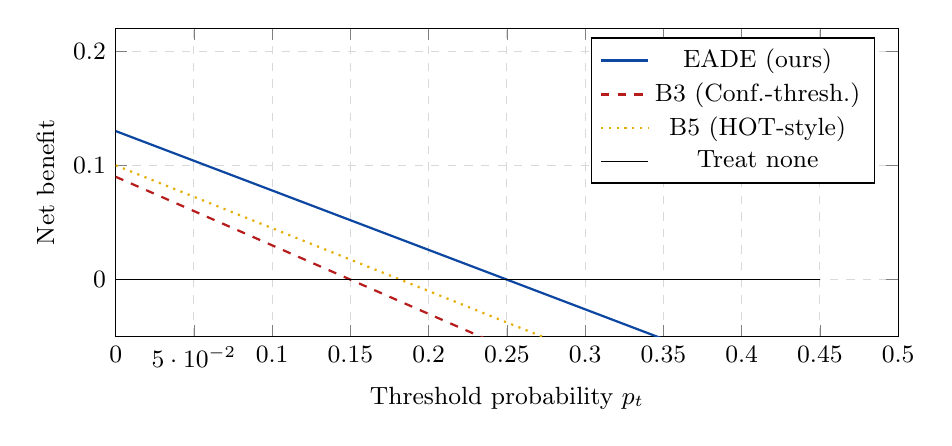
\begin{tikzpicture}
    \begin{axis}[
      width=0.95\columnwidth, height=5.5cm,
      xlabel={Threshold probability $p_t$},
      ylabel={Net benefit},
      xmin=0, xmax=0.5, ymin=-0.05, ymax=0.22,
      legend pos=north east,
      grid=major, grid style={dashed,gray!30},
      every axis/.append style={font=\small},
    ]
    \addplot[dermblue, thick, domain=0:0.45, samples=100]
      { 0.13 - 0.52*x };
    \addlegendentry{EADE (ours)}
    \addplot[dermred, dashed, thick, domain=0:0.45, samples=100]
      { 0.09 - 0.60*x };
    \addlegendentry{B3 (Conf.-thresh.)}
    \addplot[dermgold, dotted, thick, domain=0:0.45, samples=100]
      { 0.10 - 0.55*x };
    \addlegendentry{B5 (HOT-style)}
    \addplot[black, domain=0:0.45, samples=2]{ 0 };
    \addlegendentry{Treat none}
    \end{axis}
  \end{tikzpicture}
  \caption{Decision-curve analysis for malignancy referral (placeholder).
           Higher net benefit is preferable; curves below ``treat none'' are harmful.}
  \label{fig:dca}
\end{figure}

% ============================================================
\section{Robustness: DERMA-STRESS Results}
\label{sec:robustness}
% ============================================================

Table~\ref{tab:stress} summarises selective risk and guarantee violation
per stress family for EADE vs.\ B3.

\begin{table}[H]
  \centering
  \caption{%
    DERMA-STRESS summary: selective risk and guarantee violation
    $(\hat{\calR}_{\text{test}} - \alpha)$. Negative violation means guarantee
    holds; positive means broken.
  }
  \label{tab:stress}
  \renewcommand{\arraystretch}{1.2}
  \small
  \begin{tabular}{lcccc}
    \toprule
    \multirow{2}{*}{\textbf{Family}}
      & \multicolumn{2}{c}{\textbf{Selective Risk}}
      & \multicolumn{2}{c}{\textbf{Guar.\ Violation}} \\
    \cmidrule(lr){2-3}\cmidrule(lr){4-5}
      & B3 & EADE & B3 & EADE \\
    \midrule
    A Image degrad.  & -- & -- & -- & -- \\
    B Missing evid.  & -- & -- & -- & -- \\
    C Contradictory  & -- & -- & -- & -- \\
    D Dist.\ shift   & -- & -- & -- & -- \\
    E Leave-class OOD& -- & -- & -- & -- \\
    F Combined       & -- & -- & -- & -- \\
    G Operational    & n/a & n/a & n/a & n/a \\
    \bottomrule
  \end{tabular}
\end{table}

\paragraph{Guarantee violation under shift.}
Fig.~\ref{fig:violation} shows guarantee violation as a function of
distribution shift severity. This is a \emph{core reported finding}:
honest measurement of where the LTT bound breaks.

\begin{figure}[H]
  \centering
  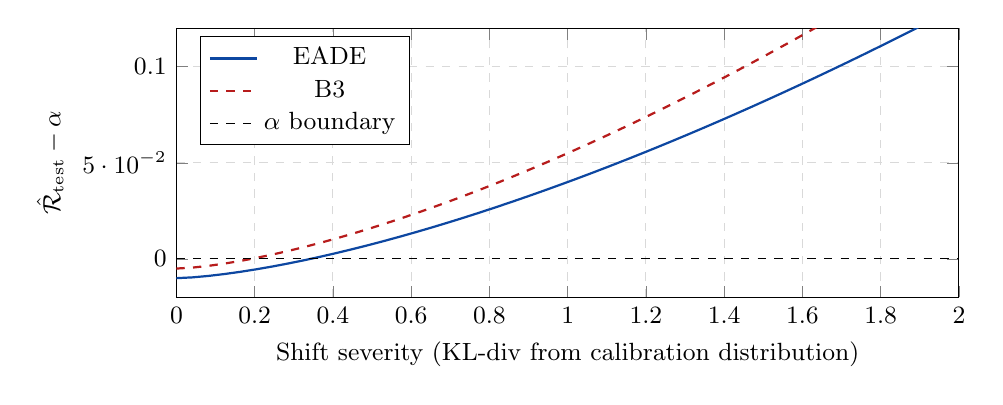
\begin{tikzpicture}
    \begin{axis}[
      width=0.95\columnwidth, height=5.0cm,
      xlabel={Shift severity (KL-div from calibration distribution)},
      ylabel={$\hat{\calR}_{\text{test}} - \alpha$},
      ymin=-0.02, ymax=0.12, xmin=0, xmax=2,
      grid=major, grid style={dashed,gray!30},
      legend pos=north west,
      every axis/.append style={font=\small},
    ]
    \addplot[dermblue, thick, domain=0:2, samples=50]
      { max(-0.01, 0.05*x^1.5 - 0.01) };
    \addlegendentry{EADE}
    \addplot[dermred, dashed, thick, domain=0:2, samples=50]
      { max(-0.005, 0.06*x^1.5 - 0.005) };
    \addlegendentry{B3}
    \addplot[black, dashed, domain=0:2, samples=2]{ 0 };
    \addlegendentry{$\alpha$ boundary}
    \end{axis}
  \end{tikzpicture}
  \caption{%
    Guarantee violation vs.\ shift severity (placeholder).
    Positive = guarantee broken. Measuring this degradation is a core contribution.
  }
  \label{fig:violation}
\end{figure}

% ============================================================
\section{Fairness Analysis}
\label{sec:fairness}
% ============================================================

\begin{table}[H]
  \centering
  \caption{%
    Per-skin-tone group coverage and miss rate (proceeded cases).
    Target: coverage $\geq 1-\alpha$; miss rate $\leq \alpha$.
    Groups with $n<30$ merged and flagged $\dagger$.
  }
  \label{tab:fairness}
  \renewcommand{\arraystretch}{1.2}
  \small
  \begin{tabular}{lccccc}
    \toprule
    \textbf{Skin-tone}
      & \textbf{$n_{\text{cal}}$}
      & \textbf{$n_{\text{test}}$}
      & \textbf{Coverage}
      & \textbf{Miss rate}
      & \textbf{Deferral} \\
    \midrule
    Level 1 (lightest) & -- & -- & -- & -- & -- \\
    Level 2            & -- & -- & -- & -- & -- \\
    Level 3            & -- & -- & -- & -- & -- \\
    Level 4            & -- & -- & -- & -- & -- \\
    Level 5            & -- & -- & -- & -- & -- \\
    Level 6 (darkest)  & -- & -- & -- & -- & -- \\
    \midrule
    \textbf{Overall}   & -- & -- & -- & -- & -- \\
    \bottomrule
  \end{tabular}
\end{table}

Subgroup results include cases where the guarantee fails for a particular
group. Wide CIs are expected for sparse groups.

% ============================================================
\section{Ablation Studies}
\label{sec:ablations}
% ============================================================

\begin{table}[H]
  \centering
  \caption{%
    Ablation on clean validation split.
    $\downarrow$AUGRC = lower is better; coverage at $\alpha=0.05$.
  }
  \label{tab:ablations}
  \renewcommand{\arraystretch}{1.2}
  \small
  \begin{tabular}{lcc}
    \toprule
    \textbf{Configuration} & \textbf{Coverage~(\%)} & \textbf{AUGRC} \\
    \midrule
    Full EADE (ours)                    & -- & -- \\
    \quad$-$ LTT safety layer           & -- & -- \\
    \quad$-$ Conformal mixed-set rule   & -- & -- \\
    \quad$-$ Acquisition estimator      & -- & -- \\
    \quad$-$ Consistency signal         & -- & -- \\
    \quad$-$ OOD signal                 & -- & -- \\
    \quad$-$ Quality signals            & -- & -- \\
    \quad Uncalibrated (no temp.\ sc.)  & -- & -- \\
    \quad Single model (no ensemble)    & -- & -- \\
    \midrule
    $\ell_{\text{miss}}=5$ sensitivity  & -- & -- \\
    $\ell_{\text{miss}}=10$ (default)   & -- & -- \\
    $\ell_{\text{miss}}=20$ sensitivity & -- & -- \\
    \bottomrule
  \end{tabular}
\end{table}

% ============================================================
\section{System Architecture}
\label{sec:architecture}
% ============================================================

DERMA-GUARD follows a modular monolith architecture with one background
worker queue. Fig.~\ref{fig:architecture} shows the end-to-end data flow.

\begin{figure}[H]
\centering
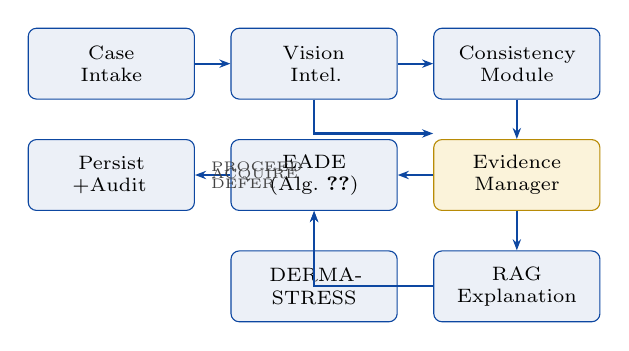
\begin{tikzpicture}[
  font=\scriptsize,
  box/.style={rectangle, draw=dermblue, fill=dermblue!8,
              rounded corners=3pt, minimum height=0.9cm,
              text width=1.9cm, align=center, inner sep=3pt},
  sbox/.style={box, fill=dermgold!15, draw=dermgold!80!black},
  arrow/.style={-{Stealth[length=4pt]}, thick, dermblue},
]
  \node[box] (intake) {Case\\Intake};
  \node[box, right=0.45cm of intake] (vision) {Vision\\Intel.};
  \node[box, right=0.45cm of vision] (consist) {Consistency\\Module};
  \node[sbox, below=0.5cm of consist] (evman) {Evidence\\Manager};
  \node[box, left=0.45cm of evman] (eade) {EADE\\(Alg.~\ref{alg:eade})};
  \node[box, left=0.45cm of eade] (persist) {Persist\\+Audit};
  \node[box, below=0.5cm of evman] (rag) {RAG\\Explanation};
  \node[box, below=0.5cm of eade] (stress) {DERMA-\\STRESS};
  \draw[arrow] (intake)--(vision);
  \draw[arrow] (vision)--(consist);
  \draw[arrow] (consist)--(evman);
  \draw[arrow] (vision)|-([yshift=2pt]evman.north west);
  \draw[arrow] (evman)--(eade);
  \draw[arrow] (eade)--(persist);
  \draw[arrow] (evman)--(rag);
  \draw[arrow] (rag)-|(eade);
  \draw[arrow] (stress)--(eade);
  \node[font=\tiny,dermgray, right=0.08cm of persist, yshift=3pt] {PROCEED};
  \node[font=\tiny,dermgray, right=0.08cm of persist] {ACQUIRE};
  \node[font=\tiny,dermgray, right=0.08cm of persist, yshift=-3pt] {DEFER};
\end{tikzpicture}
\caption{%
  DERMA-GUARD data flow. Every assessment is linked to its exact evidence
  snapshot, model, calibration, cost-matrix, and policy versions.
  Golden box = evidence management hub.
}
\label{fig:architecture}
\end{figure}

\subsection{Technology Stack}

\begin{description}[leftmargin=8pt, style=nextline, itemsep=1pt]
  \item[\textbf{Frontend.}] Next.js + React + TypeScript + Tailwind CSS.
  \item[\textbf{Backend.}] Python + FastAPI + Pydantic v2.
  \item[\textbf{Database.}] PostgreSQL + pgvector.
  \item[\textbf{Object storage.}] Local filesystem / MinIO.
  \item[\textbf{Jobs.}] Redis + RQ (one queue, one worker type).
  \item[\textbf{ML.}] PyTorch, \texttt{timm}, torchvision, scikit-learn, OpenCV.
  \item[\textbf{Conformal/UQ.}] MAPIE or $\approx$150-line in-house implementation.
  \item[\textbf{Retrieval.}] \texttt{rank\_bm25} + pgvector hybrid.
  \item[\textbf{Experiments.}] YAML configs + MLflow or plain JSON logs.
  \item[\textbf{Deployment.}] Docker Compose + GitHub Actions CI.
\end{description}

% ============================================================
\section{Limitations, Ethics, and Threats to Validity}
\label{sec:limitations}
% ============================================================

\paragraph{Statistical power.}
$\approx$786 test lesions ($\approx$50--60 melanomas); wide CIs for
rare-class metrics. All claims use bootstrap CIs.

\paragraph{Patient leakage.}
MILK10k lacks patient IDs; splits by ISIC lesion ID. Residual leakage risk
stated as a limitation.

\paragraph{Guarantee validity.}
Theorem~\ref{thm:ltt} assumes exchangeability. Under distribution shift
the guarantee may be violated; Section~\ref{sec:robustness} quantifies this.

\paragraph{Cost matrix.}
The asymmetric cost matrix is a modelling choice. Clinical validity of
specific values is not established; mandatory sensitivity sweep is reported.

\paragraph{Synthetic stress tests.}
Artificial corruptions may not reflect real clinical degradation. Multiple
severity levels and external-dataset tests are kept separate.

\paragraph{Acquisition simulation.}
``Acquiring dermoscopy'' is a controlled experiment since MILK10k already
contains paired images. Real-world acquisition-cost claims require a
prospective study.

\paragraph{Not a medical device.}
DERMA-GUARD must not be used for autonomous diagnosis.

\paragraph{LLM / RAG.}
The RAG module is decorative context, not clinical validation. LLMs cannot
alter model weights or invent citations; unsupported claims are flagged.

\paragraph{Ethics.}
All datasets are public; licences verified. No identifiable patient data
beyond approved public releases. Ethics approval required before any
real-patient data use.

% ============================================================
\section{Conclusion}
\label{sec:conclusion}
% ============================================================

We have presented DERMA-GUARD, a multimodal dermatology platform for
risk-controlled, cost-aware evidence acquisition and deferral. Its EADE
applies an expected-loss minimisation rule over a clinically asymmetric cost
matrix, calibrated via Learn-then-Test to bound malignancy miss rate among
auto-proceeded cases with probability $\geq 1-\delta$. DERMA-STRESS provides
a reproducible seven-family stress protocol; our fairness analysis
quantifies performance disparities across six skin-tone levels.

Our central claim---that explicit cost-aware acquisition and deferral
improves the reliability--coverage--cost trade-off---is a hypothesis to be
tested, not an assumed result. If the policy does not outperform baselines
on pre-registered endpoints, we report that finding and emphasise
DERMA-STRESS, the guarantee-violation analysis, and lessons learned.

\medskip\noindent\textbf{Future work.} RL-based acquisition policies;
PanDerm backbone; multi-step acquisition beyond $T_{\max}=1$;
prospective evaluation of real-world acquisition costs; extending the
conformal guarantee to covariate-shifted populations.

% ============================================================
\section*{Acknowledgements}
% ============================================================
[Funding, compute resources, and dataset licences to be acknowledged here.]

% ============================================================
\bibliographystyle{IEEEtran}
\begin{thebibliography}{99}

\bibitem{tschandl2018ham10000}
P.~Tschandl, C.~Rosendahl, and H.~Kittler,
``The HAM10000 dataset, a large collection of multi-source dermatoscopic
images of common pigmented skin lesions,''
\emph{Scientific Data}, vol.~5, p.~180161, 2018.

\bibitem{tschandl2024milk10k}
P.~Tschandl et~al.,
``MILK10k: Multimodal Image and Label Kompendium dataset,''
ISIC Archive, 2024. DOI:~10.34970/648456.

\bibitem{muller2026complementary}
O.~M{\"u}ller et~al.,
``Comparative and complementary diagnostic value of dermatoscopy
and clinical close-up photography,''
\emph{J.\ Am.\ Acad.\ Dermatol.}, DOI:~10.1016/j.jaad.2026.03.069, 2026.

\bibitem{kawahara2019derm7pt}
J.~Kawahara, S.~Daneshvar, G.~Argenziano, and G.~Hamarneh,
``Seven-point checklist and skin lesion classification using multitask
multimodal neural nets,''
\emph{IEEE J.\ Biomed.\ Health Inform.}, vol.~23, no.~2, pp.~538--546, 2019.

\bibitem{pacheco2020padufes}
A.~Pacheco et~al.,
``PAD-UFES-20: A skin lesion dataset composed of patient data and
clinical images collected from smartphones,''
\emph{Data in Brief}, vol.~32, p.~106221, 2020.

\bibitem{mehta2023hot}
S.~Mehta et~al.,
``Revamping AI models in dermatology: Hierarchical prediction, OOD alert,
and acquisition recommendation,''
arXiv:2311.01009, 2023.

\bibitem{traub2024augrc}
F.~Traub et~al.,
``Overcoming common flaws in the evaluation of selective classification
systems,''
in \emph{Proc.\ NeurIPS}, 2024. arXiv:2407.01032.

\bibitem{jiadf2025}
[Author(s) TBD],
``Joint-Individual Learning with Adaptive Decision Fusion,''
arXiv:2604.27343, 2025.

\bibitem{dermformer2025}
[Author(s) TBD],
``DermFormer: Nested multi-modal vision transformers for robust skin
cancer detection,'' 2025. [To verify before citing.]

\bibitem{zuo2025coscatnet}
Y.~Zuo et~al.,
``Adaptive multimodal fusion for multi-label skin-lesion classification
(CosCatNet),'' 2025. [To verify before citing.]

\bibitem{panderm2025}
[Author(s) TBD],
``PanDerm: A dermatology foundation model,'' 2025.
[Verify availability, licence and compute before use.]

\bibitem{geifman2017selective}
Y.~Geifman and R.~El-Yaniv,
``Selective classification for deep neural networks,''
in \emph{Proc.\ NeurIPS}, 2017. arXiv:1705.08500.

\bibitem{guo2017calibration}
C.~Guo, G.~Pleiss, Y.~Sun, and K.~Q.~Weinberger,
``On calibration of modern neural networks,''
in \emph{Proc.\ ICML}, 2017. arXiv:1706.04599.

\bibitem{lakshminarayanan2017ensembles}
B.~Lakshminarayanan, A.~Pritzel, and C.~Blundell,
``Simple and scalable predictive uncertainty estimation using deep ensembles,''
in \emph{Proc.\ NeurIPS}, 2017. arXiv:1612.01474.

\bibitem{angelopoulos2021gentle}
A.~N.~Angelopoulos and S.~Bates,
``A gentle introduction to conformal prediction and distribution-free
uncertainty quantification,''
arXiv:2107.07511, 2021.

\bibitem{angelopoulos2020raps}
A.~N.~Angelopoulos, S.~Bates, J.~Jordan, and P.~Malik,
``Uncertainty sets for image classifiers using conformal prediction (RAPS),''
arXiv:2009.14193, 2020.

\bibitem{angelopoulos2021ltt}
A.~N.~Angelopoulos et~al.,
``Learn then test: Calibrating predictive algorithms to achieve risk control,''
arXiv:2110.01052, 2021.

\bibitem{angelopoulos2022crc}
A.~N.~Angelopoulos and S.~Bates,
``Conformal risk control,''
arXiv:2208.02814, 2022.

\bibitem{mozannar2020defer}
H.~Mozannar and D.~Sontag,
``Consistent estimators for learning to defer to an expert,''
in \emph{Proc.\ ICML}, 2020. arXiv:2006.01862.

\bibitem{liu2020energy}
W.~Liu, X.~Wang, J.~Owens, and Y.~Li,
``Energy-based out-of-distribution detection,''
in \emph{Proc.\ NeurIPS}, 2020. arXiv:2010.03759.

\bibitem{lee2018mahalanobis}
K.~Lee, K.~Lee, H.~Lee, and J.~Shin,
``A simple unified framework for detecting out-of-distribution samples
and adversarial attacks,''
in \emph{Proc.\ NeurIPS}, 2018. arXiv:1807.03888.

\bibitem{lu2021fair}
C.~Lu, A.~Kumar, and J.~Hensman,
``Fair conformal predictors for applications in medical imaging,''
arXiv:2109.04392, 2021.

\bibitem{fayyad2023conformal}
J.~Fayyad et~al.,
``Empirical validation of conformal prediction for trustworthy skin
lesions classification,''
arXiv:2312.07460, 2023.

\bibitem{zoravar2025conformal}
[Author(s) TBD],
``Domain adaptive skin lesion classification via conformal ensemble
of vision transformers,''
arXiv:2505.15997, 2025.

\bibitem{shim2018joint}
H.~Shim, J.~C.~Hwang, and E.~Yang,
``Joint active feature acquisition and classification with variable-size
set encoding,''
in \emph{Proc.\ NeurIPS}, 2018.

\bibitem{valancius2023aco}
L.~Valancius et~al.,
``Acquisition conditioned oracle for nongreedy active feature acquisition,''
arXiv:2302.13960, 2023.

\bibitem{rheude2025cama}
T.~Rheude et~al.,
``Cohort-based active modality acquisition,''
arXiv:2505.16791, 2025.

\bibitem{sageagent2026}
[Author(s) TBD],
``SAGEAgent: Cost-aware sequential modality acquisition for survival prediction,''
arXiv:2607.09521, 2026.

\bibitem{vickers2006dca}
A.~J.~Vickers and E.~B.~Elkin,
``Decision curve analysis: A novel method for evaluating prediction models,''
\emph{Med.\ Decis.\ Making}, vol.~26, no.~6, pp.~565--574, 2006.

\end{thebibliography}

% ============================================================
\appendix
% ============================================================

\section{Glossary}
\label{app:glossary}

\begin{table}[H]
  \centering
  \renewcommand{\arraystretch}{1.2}
  \small
  \begin{tabular}{p{1.3cm}p{5.9cm}}
    \toprule
    \textbf{Term} & \textbf{Meaning} \\
    \midrule
    Coverage & Fraction of cases answered automatically \\
    Sel.\ risk & Error/loss rate among answered cases \\
    AUGRC & Area under generalised risk--coverage curve \\
    Conformal set & Label set containing truth with prob.\ $\geq 1-\alpha$ \\
    LTT & Learn-then-Test; high-prob.\ risk threshold \\
    OOD & Out-of-distribution input \\
    AE & Acquisition efficiency (random--oracle bounded) \\
    MSES & Minimum Sufficient Evidence Set \\
    NIR & Negative Information Rate \\
    Net benefit & Decision-curve measure at threshold $p_t$ \\
    MONET & Morphological concept annotations in MILK10k \\
    EADE & Evidence-Adaptive Decision Engine \\
    \bottomrule
  \end{tabular}
\end{table}

\section{API Endpoint Summary}
\label{app:api}

\begin{table}[H]
  \centering
  \small
  \renewcommand{\arraystretch}{1.15}
  \begin{tabular}{llp{3.6cm}}
    \toprule
    \textbf{Method} & \textbf{Endpoint} & \textbf{Purpose} \\
    \midrule
    POST & \texttt{/api/cases} & Create a case \\
    GET  & \texttt{/api/cases} & List authorised cases \\
    GET  & \texttt{/api/cases/\{id\}} & Case details \\
    POST & \texttt{/api/cases/\{id\}/assets} & Upload evidence \\
    POST & \texttt{/api/cases/\{id\}/assessments} & Request assessment \\
    GET  & \texttt{/api/assessments/\{id\}} & Status / result \\
    GET  & \texttt{/api/cases/\{id\}/timeline} & Event history \\
    POST & \texttt{/api/cases/\{id\}/reviews} & Record review \\
    GET  & \texttt{/api/policy/current} & Active policy versions \\
    POST & \texttt{/api/experiments} & Start DERMA-STRESS run \\
    GET  & \texttt{/api/experiments/\{id\}} & Experiment results \\
    \bottomrule
  \end{tabular}
\end{table}

\section{Twelve-Week Implementation Plan}
\label{app:plan}

\begin{table}[H]
  \centering
  \small
  \renewcommand{\arraystretch}{1.15}
  \setlength{\tabcolsep}{3pt}
  \begin{tabular}{clll}
    \toprule
    \textbf{Wk}
      & \textbf{M1 (ML)}
      & \textbf{M2 (Stress)}
      & \textbf{M3 (Platform)} \\
    \midrule
    1 & MILK10k EDA, labels & Novelty audit, Fam.\ A & Repo, Docker, CI \\
    2 & Splits, clin.\ baseline & Audit done; A+B & Case upload, DB \\
    3 & Derm+fused, dropout & Consistency mod.\ v1 & Background jobs \\
    4 & Ensemble, temp.\ sc. & Families C+D & Assessment, timeline \\
    5 & Conformal; B1--B3 & Fam.\ E (LCO OOD) & Review, auth \\
    6 & Acq.\ est.\ (OOF); B5--B8 & Fam.\ F; runner & Acquisition UI \\
    7 & Policy + LTT & Fairness tooling & Experiment lab \\
    8 & B4 L2D; ablations & Fam.\ G; RAG & AUGRC plots \\
    9 & Full val.\ runs & Full stress runs & Integration \\
    10 & \textbf{Test-split run} & Subgroup tables & E2E tests \\
    11 & Paper results & Paper rel.\ work & Deploy, docs \\
    12 & \multicolumn{3}{c}{\textbf{Final report, slides, demo — Submission}} \\
    \bottomrule
  \end{tabular}
\end{table}

\balance
\end{document}
%% ============================================================
%%  END OF DERMA-GUARD IEEE PAPER
%% ============================================================

